\documentclass[runningheads]{llncs}
\usepackage{hyperref}

\usepackage[T1]{fontenc}
\usepackage[utf8]{inputenc}
\usepackage[brazilian]{babel}
\usepackage{graphicx}
\usepackage{booktabs}
\usepackage{amsmath,amssymb}
\usepackage{float}
\usepackage{url}

\title{Comparação de Algoritmos Genéticos na Função de Rosenbrock: Implementação Manual e Framework \textit{pymoo}}
\titlerunning{Comparação de GAs na Função de Rosenbrock}

\author{Davi dos Santos Mattos\orcidID{119133049}}
\authorrunning{D. S. Mattos}

\institute{Universidade Federal do Rio de Janeiro, Rio de Janeiro, Brasil\\
\email{secgrad@ic.ufrj.br}}

\begin{document}
\maketitle

\begin{abstract}
Este trabalho apresenta um estudo comparativo entre três versões de algoritmo genético aplicadas à minimização da função de Rosenbrock: (i) implementação manual, (ii) implementação padrão do framework \textit{pymoo} e (iii) implementação no \textit{pymoo} com operadores configurados para aproximar a estratégia manual. O estudo utiliza seleção por torneio, recombinação BLX-$\alpha$ e mutação \textit{creep} na versão manual, com critério de parada por número máximo de avaliações da função objetivo. São analisadas a dinâmica populacional, as curvas médias de convergência em 30 execuções e a escalabilidade para diferentes dimensionalidades. Os resultados mostram superioridade consistente das abordagens baseadas em \textit{pymoo}, com destaque para a versão configurada em cenários de maior dimensionalidade.

\keywords{Algoritmo Genético \and Rosenbrock \and Metaheurísticas \and pymoo \and Otimização.}
\end{abstract}

\section{Introdução}
A função de Rosenbrock é um problema clássico para validação de métodos de otimização por apresentar um vale estreito e curvatura acentuada, o que dificulta o processo de busca do mínimo global. Nesse contexto, algoritmos genéticos (GAs) constituem uma alternativa robusta por não dependerem de informação de gradiente e por explorarem o espaço de busca de forma populacional.

Este relatório compara três configurações de GA com foco em desempenho de convergência e robustez: uma implementação manual e duas variantes no \textit{pymoo}. O objetivo é verificar o impacto dos operadores genéticos e da infraestrutura de execução sobre a qualidade das soluções finais.

\section{Metodologia}
* Todo o código utilizado e implementado está disponível através do \href{https://colab.research.google.com/drive/1EyCrbTjGR4i4W6h1q3MaOLaOT6038weT?usp=sharing}{Google Colab}.

\subsection{Problema de otimização}
A função objetivo utilizada foi a função de Rosenbrock em dimensão $d$:
\begin{equation}
    f(\mathbf{x}) = \sum_{i=1}^{d-1} \left[100(x_{i+1} - x_i^2)^2 + (x_i - 1)^2\right].
\end{equation}
O mínimo global ocorre em $\mathbf{x}^* = (1,\ldots,1)$, com $f(\mathbf{x}^*) = 0$.

\subsection{Algoritmo genético manual}
A implementação manual foi construída com indivíduos reais no intervalo $[-5,10]$ e os seguintes componentes:
\begin{itemize}
\item Seleção por torneio;
\item Cruzamento BLX-$\alpha$ (com $\alpha=0{,}3$);
\item Mutação \textit{creep} gaussiana (taxa de mutação de 0,05 e $\sigma=0{,}1$);
\item Critério de parada por número máximo de avaliações da função (até 100.000).
\end{itemize}

\subsection{Configurações no \textit{pymoo}}
Foram avaliadas duas variantes:
\begin{itemize}
\item \textbf{GA padrão}: configuração nativa do \textit{pymoo}, alterando apenas o tamanho da população e o limite de avaliações;
\item \textbf{GA configurado}: versão com seleção por torneio , cruzamento BLX-$\alpha$ e mutação \textit{creep}, mantendo a eliminação de duplicatas (versão criada com auxílio de LLM).
\end{itemize}

\subsection{Protocolo experimental}
Os experimentos seguiram os mesmos limites de busca e tamanho populacional ($N=100$), com análise em duas etapas:
\begin{itemize}
\item Análise da dinâmica populacional em 2D para 1, 2.500, 5.000 e 100.000 avaliações;
\item Comparação estatística por curva média em 30 execuções para 2, 5, 10 e 30 dimensões.
\end{itemize}
As curvas são apresentadas em escala logarítmica no eixo de \textit{fitness}.

\section{Resultados}
\subsection{Evolução da população (2D)}
As Figuras~\ref{fig:pop1}--\ref{fig:pop100k} ilustram a distribuição da população sobre as curvas de nível da função de Rosenbrock. Observa-se que a população inicia dispersa e, ao longo das avaliações, concentra-se progressivamente na região do mínimo global.

\begin{figure}[H]
\centering
\begin{minipage}{0.48\textwidth}
\centering
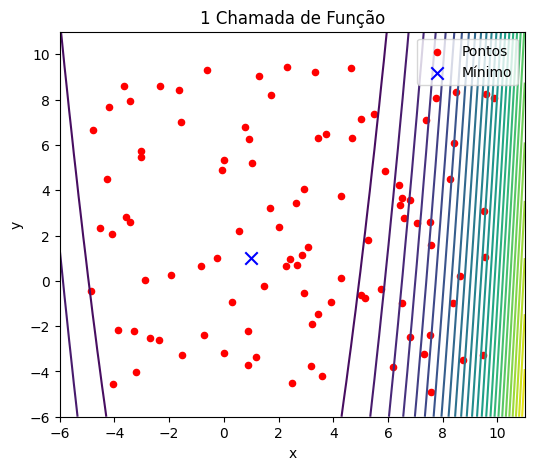
\includegraphics[width=\textwidth]{comportamento_1.png}
\caption{População com 1 avaliação.}
\label{fig:pop1}
\end{minipage}
\hfill
\begin{minipage}{0.48\textwidth}
\centering
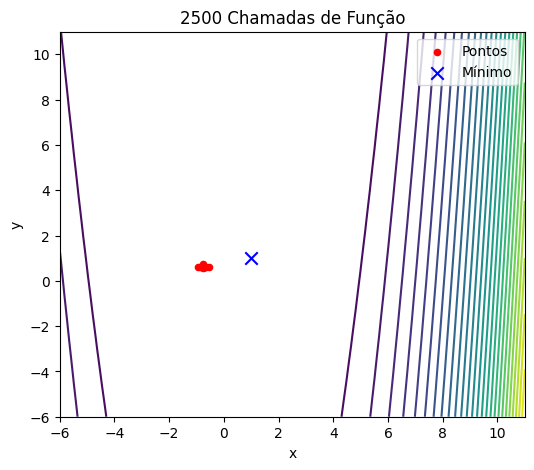
\includegraphics[width=\textwidth]{comportamento_2500.png}
\caption{População com 2.500 avaliações.}
\label{fig:pop2500}
\end{minipage}
\end{figure}

\begin{figure}[H]
\centering
\begin{minipage}{0.48\textwidth}
\centering
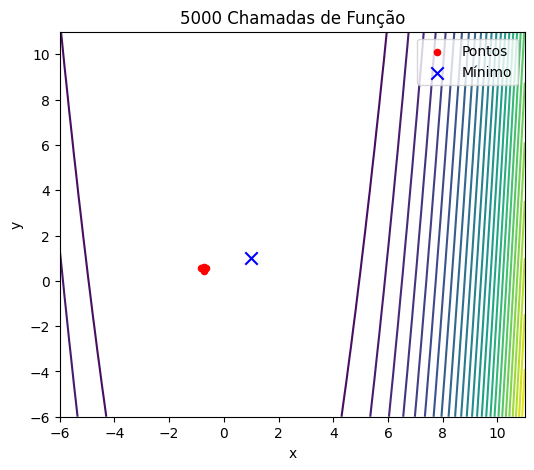
\includegraphics[width=\textwidth]{comportamento_5000.png}
\caption{População com 5.000 avaliações.}
\label{fig:pop5000}
\end{minipage}
\hfill
\begin{minipage}{0.48\textwidth}
\centering
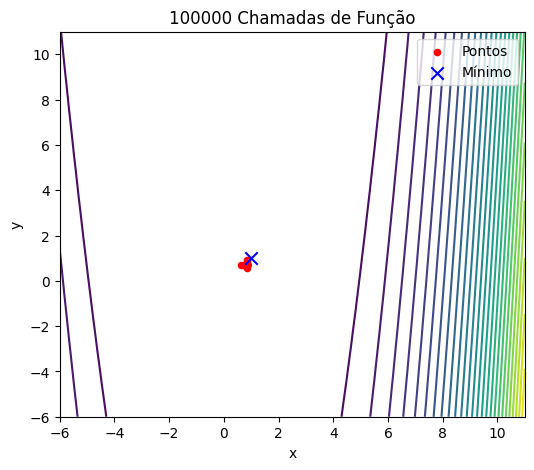
\includegraphics[width=\textwidth]{comportamento_100000.png}
\caption{População com 100.000 avaliações.}
\label{fig:pop100k}
\end{minipage}
\end{figure}

\subsection{Comparação em 2D}
A Figura~\ref{fig:conv2ga} compara o GA manual e o GA padrão do \textit{pymoo} em 30 execuções. Nota-se uma convergência significativamente mais rápida do \textit{pymoo}, atingindo valores de \textit{fitness} menores em um menor número de avaliações.

\begin{figure}[H]
\centering
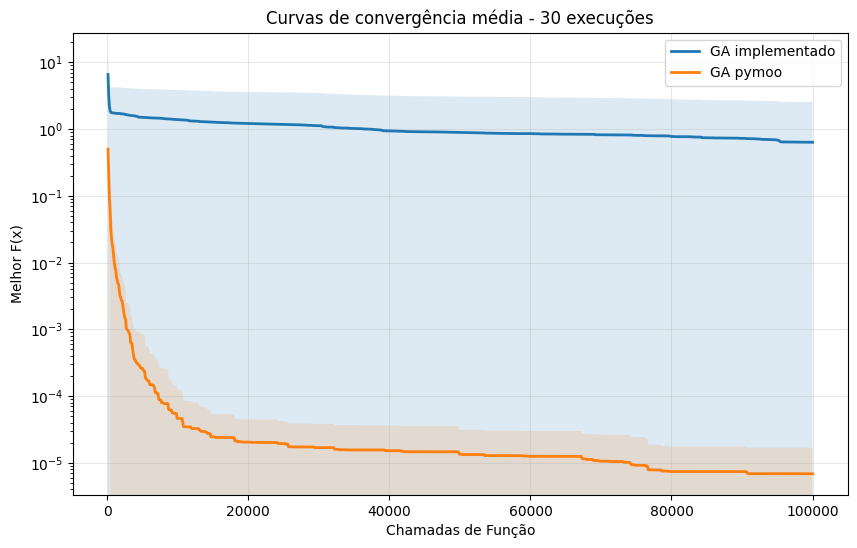
\includegraphics[width=0.78\textwidth]{convergencia_media_2d_2_ga.png}
\caption{Curvas médias de convergencia (30 execuções) para GA manual e GA padrão do \textit{pymoo} em 2D.}
\label{fig:conv2ga}
\end{figure}

A Figura~\ref{fig:conv2d} inclui também a versão configurada do \textit{pymoo}. Em 2D, o GA padrão e o GA configurado apresentam desempenho competitivo entre si, ambos superiores ao GA manual.

\begin{figure}[H]
\centering
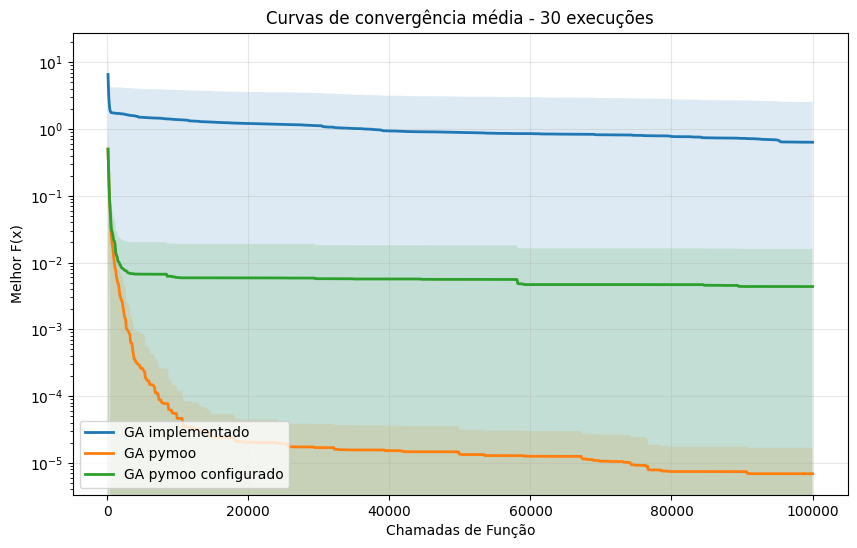
\includegraphics[width=0.78\textwidth]{convergencia_media_2d.png}
\caption{Curvas médias de convergência (30 execuções) para as três abordagens em 2D.}
\label{fig:conv2d}
\end{figure}

\subsection{Tabela final de comparação }
A Tabela~\ref{tab:item6_2d} apresenta a comparação entre as três versões avaliadas em 2D, com 30 execuções. O \textit{fitness} final considerado é o valor do melhor indivíduo (\textit{best}) na última geração de cada execução.

\begin{table}[H]
\centering
\caption{Resumo estatístico final em 2D (30 execuções): GA implementado, GA \textit{pymoo} e GA \textit{pymoo} configurado.}
\label{tab:item6_2d}
\scriptsize
\setlength{\tabcolsep}{4pt}
\resizebox{\textwidth}{!}{%
\begin{tabular}{@{}lcccccc@{}}
\toprule
Versão & Média final & Desvio padrão final & Mediana final & Execução mediana & Indivíduo mediano & \textit{Fitness} da execução mediana \\
\midrule
GA implementado & 0,635246 & 1,91969 & 0,0377446 & 4 & [0,805007, 0,64809] & 0,0380226 \\
GA \textit{pymoo} & 6,87271e-06 & 9,95935e-06 & 2,71525e-06 & 7 & [1,001728, 1,003463] & 2,98872e-06 \\
GA \textit{pymoo} configurado & 0,00437722 & 0,0116346 & 2,70014e-05 & 25 & [1,005664, 1,011365] & 3,20797e-05 \\
\bottomrule
\end{tabular}
}
\end{table}

Pelos resultados da Tabela~\ref{tab:item6_2d}, a versão que se sobressai em 2D é o \textbf{GA \textit{pymoo}} em média final, enquanto o \textbf{GA implementado} apresenta a menor mediana final. O \textbf{GA \textit{pymoo} configurado} aparece como alternativa intermediária, com baixa variabilidade entre execuções.

\section{Comparação por Dimensionalidade }
Neste item, cada dimensionalidade é apresentada como subitem com: (i) curva de convergência média de 30 execuções, (ii) interpretação sobre qual versão se sobressai e (iii) tabela com média, desvio padrão, mediana, execução mediana, indivíduo mediano e \textit{fitness} da execução mediana.

Os gráficos de convergência média mostram, para cada número de avaliações da função objetivo, o comportamento médio do melhor \textit{fitness} obtido ao longo das 30 execuções. A linha principal resume a tendência central de cada algoritmo, enquanto a faixa sombreada indica a dispersão dos resultados entre as execuções, permitindo avaliar simultaneamente velocidade de convergência e estabilidade.

\subsection{Dimensão 5D}
\begin{figure}[H]
\centering
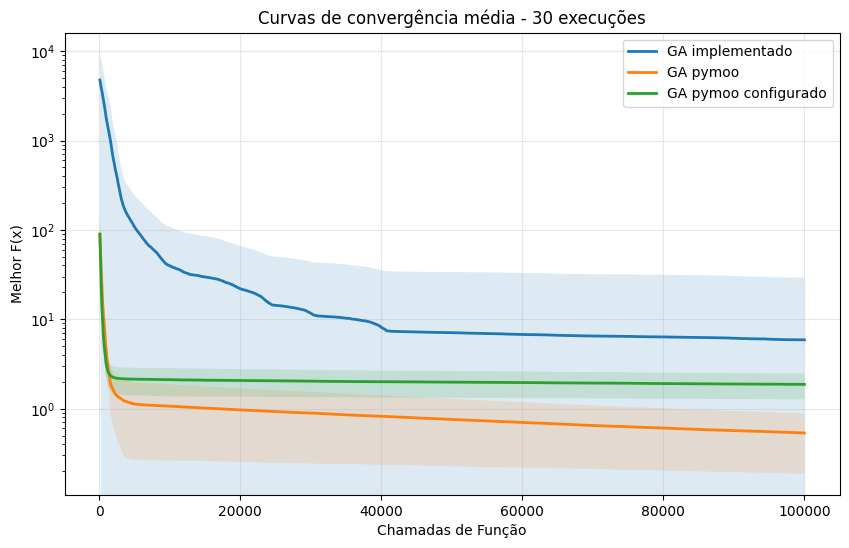
\includegraphics[width=0.78\textwidth]{convergencia_media_5d.png}
\caption{Curvas médias de convergência (30 execuções) em 5D.}
\label{fig:conv5d}
\end{figure}

Em 5D, a versão que mais se sobressai é o \textbf{GA \textit{pymoo}}, pois apresenta o menor \textit{fitness} médio final e também a menor mediana final entre as três abordagens.

\begin{table}[H]
\centering
\caption{Resumo estatístico final em 5D (30 execuções).}
\label{tab:resumo_5d}
\scriptsize
\setlength{\tabcolsep}{4pt}
\resizebox{\textwidth}{!}{%
\begin{tabular}{@{}lcccccc@{}}
\toprule
Versão & Média final & Desvio padrão final & Mediana final & Execução mediana & Indivíduo mediano & \textit{Fitness} da execução mediana \\
\midrule
GA implementado & 5,88677 & 23,3532 & 0,712228 & 7 & [0,871666, 0,763261, 0,581052, 0,342265, 0,113116] & 0,685854 \\
GA \textit{pymoo} & 0,533806 & 0,346973 & 0,657363 & 9 & [0,880485, 0,776246, 0,608622, 0,372583, 0,131571] & 0,620673 \\
GA \textit{pymoo} configurado & 1,86835 & 0,597288 & 1,98421 & 8 & [0,669392, 0,445484, 0,208888, 0,049786, 0,002367] & 1,9609 \\
\bottomrule
\end{tabular}
}
\end{table}

\subsection{Dimensão 10D}
\begin{figure}[H]
\centering
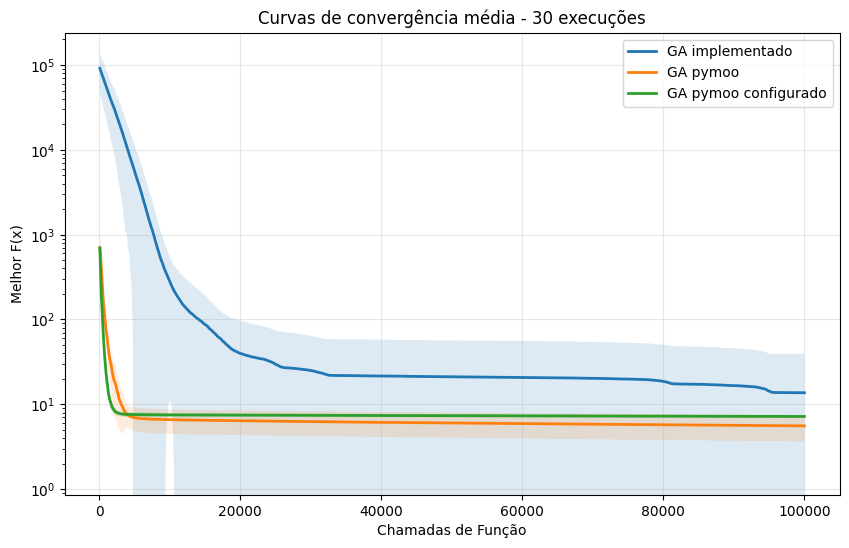
\includegraphics[width=0.78\textwidth]{convergencia_media_10d.png}
\caption{Curvas médias de convergência (30 execuções) em 10D.}
\label{fig:conv10d}
\end{figure}

Em 10D, novamente o \textbf{GA \textit{pymoo}} se sobressai em média final, enquanto o GA implementado apresenta a menor mediana final. A versão configurada permanece competitiva, mas não supera o GA \textit{pymoo} padrão neste conjunto de execuções.

\begin{table}[H]
\centering
\caption{Resumo estatístico final em 10D (30 execuções).}
\label{tab:resumo_10d}
\small
\setlength{\tabcolsep}{3pt}
\resizebox{\textwidth}{!}{%
\begin{tabular}{@{}lcccccc@{}}
\toprule
Versão & Média final & Desvio padrão final & Mediana final & Exec. mediana & Indivíduo mediano & \textit{Fitness} execução mediana \\
\midrule
GA implementado & 13,6985 & 25,5053 & 5,23377 & 16 & [8.78e-01, 7.75e-01, ..., 1.01e-02, 6.75e-04] & 5,24958 \\
GA \textit{pymoo} & 5,57747 & 1,92067 & 6,05638 & 30 & [0,803, 0,647, ..., 0,011, 0,00124] & 6,05737 \\
GA \textit{pymoo} configurado & 7,19376 & 0,281863 & 7,28029 & 21 & [5.84e-01, 3.47e-01, ..., 1.02e-02, -2.43e-04] & 7,27686 \\
\bottomrule
\end{tabular}
}
\end{table}

\subsection{Dimensão 30D}
\begin{figure}[H]
\centering
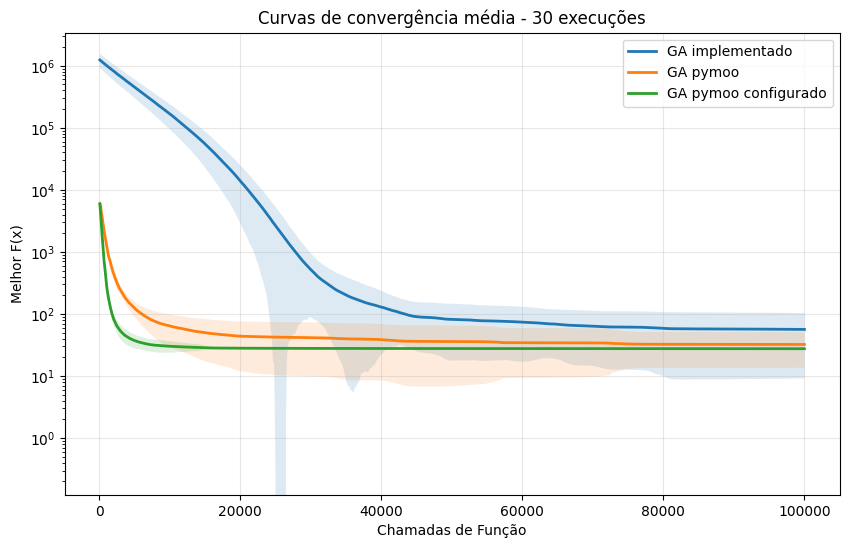
\includegraphics[width=0.78\textwidth]{convergencia_media_30d.png}
\caption{Curvas médias de convergência (30 execuções) em 30D.}
\label{fig:conv30d}
\end{figure}

Em 30D, o \textbf{GA \textit{pymoo} configurado} se torna a melhor alternativa, com menos variabilidade. Porém o \textbf{GA \textit{pymoo}} continua sendo competitivo com uma melhor Mediana e Fitness da exeução mediana.

\begin{table}[H]
\centering
\caption{Resumo estatístico final em 30D (30 execuções).}
\label{tab:resumo_30d}
\small
\setlength{\tabcolsep}{3pt}
\resizebox{\textwidth}{!}{%
\begin{tabular}{@{}lcccccc@{}}
\toprule
Versão & Média final & Desvio padrão final & Mediana final & Exec. mediana & Indivíduo mediano & \textit{Fitness} execução mediana \\
\midrule
GA implementado & 56,3063 & 47,1505 & 26,7902 & 21 & [0,645, 0,420, ..., 0,0101, 0,00111] & 26,8206 \\
GA \textit{pymoo} & 32,2322 & 18,6446 & 26,7791 & 23 & [0,675, 0,445, ..., 0,00993, 5,06e-04] & 26,7267 \\
GA \textit{pymoo} configurado & 27,5255 & 0,567078 & 27,6556 & 5 & [0,434, 0,182, ..., 0,0156, 2,23e-04] & 27,663 \\
\bottomrule
\end{tabular}
}
\end{table}

\subsection{Dimensão 30D (Implementado + pymoo padrão)}

Em 30D, a comparação entre o GA implementado e o GA \textit{pymoo} padrão confirma a vantagem do \textit{pymoo} em média final e em mediana final.

\begin{table}[H]
\centering
\caption{Resumo estatístico final em 30D (30 execuções): GA implementado e GA \textit{pymoo}.}
\label{tab:resumo_30d_2}
\small
\setlength{\tabcolsep}{3pt}
\resizebox{\textwidth}{!}{%
\begin{tabular}{@{}lcccccc@{}}
\toprule
Versão & Média final & Desvio padrão final & Mediana final & Exec. mediana & Indivíduo mediano & \textit{Fitness} execução mediana \\
\midrule
GA implementado & 56,3063 & 47,1505 & 26,7902 & 21 & [0,645, 0,420, ..., 0,0101, 0,00111] & 26,8206 \\
GA \textit{pymoo} & 32,2322 & 18,6446 & 26,7791 & 23 & [0,675, 0,445, ..., 0,00993, 5,06e-04] & 26,7267 \\
\bottomrule
\end{tabular}
}
\end{table}

\subsection{Síntese}
Considerando 5D, 10D e 30D, a versão que se sobressai de forma consistente é o \textbf{GA \textit{pymoo}} em 5D e 10D, enquanto o \textbf{GA \textit{pymoo} configurado} apresenta a menor média final em 30D. Em termos de mediana, o GA \textit{pymoo} permanece competitivo, mas o desempenho relativo varia com a dimensionalidade.

\section{Conclusão}
Este trabalho comparou três variantes de algoritmo genético para a minimização da função de Rosenbrock. A análise experimental mostrou que:
\begin{enumerate}
\item O GA manual apresenta a pior taxa de convergência média;
\item O GA padrão do \textit{pymoo} melhora substancialmente os resultados em 2D, 5D e 10D;
\item O GA configurado no \textit{pymoo} apresenta o melhor desempenho em 30D.
\end{enumerate}

Como extensão futura, recomenda-se avaliar a sensibilidade de hiperparâmetros (pressão de torneio, taxa de mutação e $\alpha$ do BLX), além de incluir testes estatísticos formais (por exemplo, Wilcoxon ou Friedman) para consolidar a comparação entre os métodos.

\begin{thebibliography}{99}

\bibitem{takahashi2023}
Takahashi, R.H.C.: Notas de Aula: Otimização Escalar e Vetorial -- Volume 2: Otimização Escalar.
Departamento de Engenharia Elétrica, Universidade Federal de Minas Gerais, Belo Horizonte (2023).

\bibitem{colab}
Mattos, D.S.: Código do trabalho no Google Colab.
\url{https://colab.research.google.com/drive/1QzpCkviWcmNqncEVkiM7mFcWjVB7TdL_?usp=sharing}

\bibitem{vlse}
VLSE: Virtual Library of Simulation Experiments.
\url{https://www.sfu.ca/~ssurjano/optimization.html}, último acesso em 06/04/2026.

\bibitem{slides_carolina}
Marcelino, C.G.: Slides de aula da disciplina de Otimização com Metaheurísticas.
Universidade Federald do Rio de Janeiro,
2026/1.

\bibitem{pymoo}
Blank, J., Deb, K.: \textit{pymoo: Multi-Objective Optimization in Python}.
IEEE Access 8, 89497--89509 (2020).
\url{https://pymoo.org/}

\bibitem{rosenbrock}
Rosenbrock, H.H.: \textit{An Automatic Method for Finding the Greatest or Least Value of a Function}.
The Computer Journal 3(3), 175--184 (1960).

\end{thebibliography}

\end{document}